\cotefile{156-6}

\scanpage{6}\mspage{5}
\deleted{une figure a}

Pour \deleted{toute} figure $F$, $\operatorname{Multomb}(F)$ \inserted{est appelé} \deleted{\unsure{de|la}} la \uline{grande} \uline{multiombre} de $F$, ou la $\mathcal{M}$-multiombre de $\mathbb{F}$. \deleted{On} C'est en fait une figure ensembliste dans $\mathcal{M}$\inserted{indexée fidèlement par $\widetilde F$ (le déployement de $F$)}, et dont la connaissance implique celle de $F$.

\inserted{Jusqu'à présent il n'était pas question de $\mathcal{L}$.} Utilisant \deleted{d'autre part} \inserted{\unsure{maintent|maintnt|maintenant}} l'application
\[
\mathcal{L}\hookrightarrow\mathcal{M},
\]
et les applications images inverses correspondantes
\[
\begin{aligned}
\unsure{\mathcal{P}|\mathscr{P}|\mathfrak{P}}(\mathcal{M})&\longrightarrow\mathcal{P}(\mathcal{L})\\
\operatorname{Fig}(\mathcal{M})&\rightharpoonup\operatorname{Fig}(\mathcal{L})
\end{aligned}
\]
on trouve, en composant avec 1.6 a)b)
\[
\left\{\begin{aligned}
\text{a)}\quad \unsure{\mathcal{F}|\mathfrak{F}}&\mathrel{\deleted{\lhook}\!\longrightarrow}\mathcal{P}(\mathcal{L})&
 F&\longmapsto\operatorname{omb}(F)\\
\text{b)}\quad \mathcal{F}&\mathrel{\deleted{\lhook}\!\longrightarrow}\operatorname{Fig}(\mathcal{L})&
 F&\longmapsto\operatorname{mul\unsure{t|\deleted{t}}omb}(F),
\end{aligned}\right.\tag*{(1.9)}
\]
% The t in the displayed multomb is heavily overwritten: live/retraced t versus deleted t remains unresolved.
dont la première n'a aucune raison d'être injective, \unsure{la seconde|le second} par contre a une tendance à l'être$\times$ \deleted{on ne rien} \inserted{On} appelle $\operatorname{omb}(F)$ la \uline{petite ombre} de $F$, ou simplement son ombre quand une confusion semble exclue, et de $\overline m$ pour $\operatorname{multomb}$, la (\uline{petite}) \uline{multiombre de la} figure $F$.

\scanpage{7}\mspage{6}
Ainsi, l'ombre d'une figure est formée des lieux qui la raffinent -- on dit aussi que ce sont les \uline{lieux ``de la figure}'' (à ne pas confondre, avec les strates de la figure qui sont des lieux). La \unsure{\deleted{om}multiombre|multiombre} est donc \unsure{formé|formée} des ombres de ses strates, elle est indexée par le déployement $\widetilde F$, ensemble des strates de $F$, la relation d'\deleted{\unsure{d'ordre|d'inclu}}\inserted{\unsure{inclusion}} de la figure ensembliste n'étant autre que la relation d'\unsure{incidences|incidence} entre strates de $F$, ie. la relation \unsure{de|dans} $\widetilde F$ induite par $\leq$ \unsure{de|dans} $\mathcal M$ (ou par $\ll$ au choix, ça revient au $\overline m$). Alors qu'une figure ne se réconstitue pratiquement jamais à partir de son ombre, elle se réconstitue pourtant \deleted{\unsure{à|d}}\inserted{s}ouvent (cas des ``\unsure{\deleted{a}A|A}teliers ensemblistes'') \deleted{de}\inserted{à} partir de sa multiombre. Nous y reviendrons.

\S{} Il y a lieu de parler des relations d'ordre canoniques

\scanpage{8}\mspage{7}
\[
\begin{aligned}
\leq,\quad\ll,\quad\preccurlyeq&\qquad\text{relations d'ordre}\\
&\qquad\text{\unsure{de|dans} }\unsure{\mathcal{F}|\mathfrak{F}}
\end{aligned}\tag*{(1.10).}
\]
et les relations induites dans $\mathcal{M}$
\[
\leq,\quad\ll\quad\text{dans }\mathcal{M}\tag*{(1.11)}
\]
% slanted
\margin{\uline{NB} \unsure{Les|les} relations d'ordre induites par $\leq$, $\ll$ sur $\mathcal{L}$ sont discrètes.}
[nb la relation d'ordre $\preccurlyeq$ induite dans $\mathcal{M}$ est moins importante, comme structure spécifique dans $\mathcal{M}$].

% slanted
\margin{\uline{NB} $G\leq F\Longrightarrow G\ll F$ : une sous-figure de $F$ raffine $F$}
\begin{center}
\begin{tabular}{@{}l@{\quad}p{.64\linewidth}@{}}
$\deleted{F}G\deleted{\unsure{\ll|<}}\leq\deleted{G}F$ & $\deleted{F}G$ est dit une \uline{sous}-\uline{figure} de $\deleted{G}F$\\
& (Si $\deleted{F}G\inserted{=X}\in\mathcal{M}$, c'est donc une \uline{strate} de $\deleted{G}F$)\\[.45em]
$G\ll F$ & $G$ est dit un \uline{raffinement} de $F$\\
& (si $G=\unsure{x|X}\in\mathcal{M}$, c'est donc un élément de la grande o\unsure{m|\deleted{o}m|\deleted{m}m}bre de $F$)\\[.45em]
$G\preccurlyeq F$ & $G$ est dit une \uline{subdivision} de $F$,\\
& on dit que la figure $G$ subdivise la figure $F$.
\end{tabular}
\end{center}

Je note enfin deu\deleted{\unsure{q|x}}x autres relations importantes \deleted{dans} entre figures:
\[
\left\{\begin{aligned}
F\text{ et }G&\quad\text{\uline{compatibles}}\\
F\text{ et }G&\quad\text{\uline{disjoints}}\qquad,
\end{aligned}\right.\tag*{(1.12)}
\]
qui l'une et l'autre peuvent s'exprimer en termes de la relation d'ordre $\leq$:

$F$ et $G$ compatibles: ce sont des sous figures d'une $\overline m$ figure, \unsure{i..e|i.e} $\{F,G\}$ majoré pour $\leq$;

$F$ et $G$ disjoint: $F$ et $G$ compatibles, et leur

\scanpage{9}\mspage{8}
$\inf$ dans $\unsure{\mathcal{F}|\mathfrak{F}}$ est $\varnothing_{\mathcal{F}}$, le plus petit élément. de $\mathcal{F}$ ou \uline{figure vide}. Ainsi
\[
F\text{ et }G\text{ disjoints}\quad\Longrightarrow\quad F\text{ et }G\text{ compatibles}.
\]

On a, par les axiomes:
\[
\begin{aligned}
&&\deleted{\text{tout}}\quad\inserted{\operatorname{omb}(F)\text{ et }\operatorname{omb}(G)}\\
F\text{ et }G\text{ disjoints}&\quad\Longleftrightarrow\quad&\deleted{\operatorname{omb}(F)\cap\operatorname{omb}(G)\unsure{=}}\\
&&\text{sont ``disjoints'' \unsure{au|un} sens}\\
&&\text{suivant: ils sont \unsure{disjoint|disjoints}}\\
&&\text{ensemblistement i.e.}\\
&&\operatorname{omb}(F)\cap\operatorname{om}(G)=\varnothing,\ \text{et}\\
&&\text{tout élément de }\operatorname{omb}(F)\text{ est}\\
&&\text{compatible avec tout elt}\\
&&\text{de }\operatorname{om}(G)
\end{aligned}\tag*{(1.13)}
\]
-- i.e. deux figures sont disjointes ssi elles n'ont pas de lieu \unsure{communs|commun}, et tout lieu de l'une est \deleted{disjoint} \inserted{\deleted{com} disjoint} (au sens de l\unsure{\deleted{a}|a}\inserted{'}\deleted{théorie}atelier) de tout lieu de l'autre;

Cela montre que les relations de \deleted{\unsure{dis|disj}}compatibilité et de disjonction sont importantes aussi dans les \deleted{\unsure{en des|en de}} \inserted{sous-}ensembles $\mathcal{M},\mathcal{L}$ de $\mathcal{F}$. Dans le cas des ateli\unsure{ers|\deleted{er}ers|\deleted{ers}ers} ensemblistes, ces relations sont ``triviales'' sur $\mathcal{L}$: deux lieux sont tjrs \deleted{disjoints} \inserted{compatibles}, et disjoints ssi ils sont distincts. Par contre, même dans le cas ensembliste et $\overline m$ modéré, la relation

\scanpage{10}\mspage{9}
\makeatletter\tagsleft@true\makeatother
de \uline{compatibilité} dans $\unsure{\mathcal{M}|M}$ est une \deleted{notion} relation importante, qui se \unsure{surajoute|surrajoute} aux relations $\underset{\mathcal{M}}{\leq}$, $\underset{\mathcal{M}}{\ll}$. Moralement, pour récupérer l'atelier (à iso unique près) il suffit de connaitre sur $\mathcal{M}$ ces deux relations d'ordre, et la relation de compatibilité.
% slanted
\margin{au moins dans le cas modéré}

Les relations \deleted{\unsure{suivantes}} \inserted{(compatibilité, disjonction)} sont si importantes, qu'elles méritent chacune une notation lapidaire. Je propose
\[
\deleted{F\parallel G}\qquad F\parallel G \tag*{(1.14)}
\]
pour la disjonction, et
\[
\deleted{F\unsure{\mathrel{\tikz[baseline=0pt,x=1em,y=1em]{\draw (-.38,.62)--(.38,.25)--(-.43,-.10); \draw (.34,.62)--(-.32,.25)--(.38,-.10);}}|\mathrel{\tikz[baseline=0pt,x=1em,y=1em]{\draw (-.44,.26)--(0,.58)--(.44,.26)--(0,-.06)--cycle; \draw (0,.58)--(0,-.06);}}}G}\qquad F\mathrel{\tikz[baseline=0pt,x=1em,y=1em]{\draw (-.44,.26)--(0,.58)--(.44,.26)--(0,-.06)--cycle; \draw (0,.58)--(0,-.06);}} G\quad\text{ou}\quad
\tikz[baseline=(fg.base)]{\node[inner sep=1pt] (fg) {$F\mathrel{\tikz[baseline=0pt,x=1em,y=1em]{\draw (-.38,.62)--(.38,.25)--(-.43,-.10); \draw (.34,.62)--(-.32,.25)--(.38,-.10);}} G$}; \draw ([shift={(70:2.12em and 1.40em)}]fg.center) arc[start angle=70,end angle=410,x radius=2.12em,y radius=1.40em];}
\tag*{(1.15)}
\]
pour la compatibilité (NB $\mathrel{\tikz[baseline=0pt,x=1em,y=1em]{\draw (-.38,.62)--(.38,.25)--(-.43,-.10); \draw (.34,.62)--(-.32,.25)--(.38,-.10);}}$ est plus rapide \unsure{:|à} écrire que $\mathrel{\tikz[baseline=0pt,x=1em,y=1em]{\draw (-.44,.26)--(0,.58)--(.44,.26)--(0,-.06)--cycle; \draw (0,.58)--(0,-.06);}}$, $\unsure{\mathrel{\tikz[baseline=0pt,x=1em,y=1em]{\draw (-.12,.56)--(-.48,.25)--(-.12,-.02); \draw (.10,.56)--(.49,.25)--(.13,-.03); \draw (-.32,.51)--(-.59,.25)--(-.28,.18)--(.20,.30)--(.49,.25); \draw (-.28,.18)--(.02,.45); \draw (.26,.55)--(.50,.25);}}|\deleted{\mathrel{\tikz[baseline=0pt,x=1em,y=1em]{\draw (-.12,.56)--(-.48,.25)--(-.12,-.02); \draw (.10,.56)--(.49,.25)--(.13,-.03); \draw (-.32,.51)--(-.59,.25)--(-.28,.18)--(.20,.30)--(.49,.25); \draw (-.28,.18)--(.02,.45); \draw (.26,.55)--(.50,.25);}}}}$ mais est moins suggestif de l'idée combinatoire exprimée.

On n'a rien dit pour l'instant au sujet de la relation $\deleted{\ll}\preccurlyeq$ de raffinement sur $\unsure{\mathcal{F}|\mathfrak{F}}$. Elle est formellement de nature plus délicate, et est la notion la plus spécifique dans l'``Algèbre des figures''. La signification géométrique s'éclaire par les \unsure{exemples|exemple}, et les axiomes que \unsure{ceux-|ceux}%

\scanpage{11}\mspage{10}%
ci inspirent.

\uline{Axiomes}\quad On peut prendre pour ens de base \unsure{ds|d'} une axiomatique des ateliers, soit $\unsure{\mathcal{F}|\mathfrak{F}}$, soit $\unsure{\mathcal{M}|M}$, soit $\mathcal{L}$. On trouve des données les plus simples sur $\mathcal{F}$, les \deleted{plus} \unsure{sophistiquées|sophistiqués} sur $\mathcal{L}$. Par contre, les axiomes essentiels sont les moins transparents quand on \unsure{entre|reste} plus ou moins dans $\mathcal{F}$, le plus transparent quand on travaille dans $\mathcal{L}$ (ou peut-être pareil pour $\mathcal{M}$ ?).

\uline{Sur $\mathcal{F}$}, on peut prendre comme structure de base, au choix
\[
\left\{\begin{aligned}
 &\text{a)}\ \leq,\ \ll\\
 &\text{b)}\ \leq,\ \preccurlyeq \quad \longleftarrow\\
 &\text{c)}\ \ll,\ \deleted{\unsure{F|\mathcal{F}}}\quad
 \underbrace{\text{et}\quad\mathcal{F}\longrightarrow\mathrm{P}(\mathcal{F})}_{
 \begin{smallmatrix}
 \text{i.e. la \uline{relation}}\\[-1pt]
 \text{\uline{d'incidence}}\\
 \text{``$F$ est une strate de $G$''}\\
 \text{(i.e. $F\in\mathcal{M}$ \uline{et} $F\leq G$)}
 \end{smallmatrix}}
\end{aligned}\right.
\quad
\begin{aligned}
 &\text{(notée }F\longmapsto\widetilde F,\ \text{le}\\
 &\text{déployement de }F\\
 &\text{vu comme partie de }\mathcal{F}\text{)}\\
 &\text{\deleted{i.e. la \deleted{\unsure{description|désignation}} \inserted{relation \unsure{d'inc.|d'inc}}}}
\end{aligned}
\tag*{(1.16)}
\]
% The upper replacement relation d'inc. was inserted above the canceled noun;
% the encompassing i.e. phrase and its replacement were subsequently canceled.
% slanted; the arrow beside b) points from this dated note to that row.
\margin{(\unsure{20-juin|20. juin}) Non, par mon nouveau point de vue ça n'implique plus $\ll$}

\deleted{Je} Avant de préciser \unsure{ces points|ce point}, je vais grouper dans un diagramme les six relations fondamentales dans $\mathcal{F}$, en écrivant
\[
\unsure{F|\mathbb{F}}\triangleleft G\quad
\underset{\unsure{\mathrm{par}}}{\overset{\mathrm{dfn}}{\Longleftrightarrow}}\quad
\text{``$F$ incident à $G$''}\quad\text{i.e.}\quad F\leq G\ \text{et}\ F\in\mathcal{M}
\tag*{(1.17)}
\]

\scanpage{12}\mspage{11}
\diagram{%
\[
\vcenter{\hbox{\begin{tikzcd}[ampersand replacement=\&,row sep=1.25em,column sep=.2em,
execute at end picture={
\draw ([xshift=-.45em,yshift=1em]leq.north west) -- ([xshift=.8em,yshift=.15em]leq.north east);
\draw ([xshift=.55em,yshift=.26em]leq.north east) -- ([xshift=.75em,yshift=-.95em]ltlt.south east) -- ([xshift=-.9em,yshift=-.1em]ltlt.south west);
\draw ([xshift=-.65em,yshift=.93em]leq.north west) -- ([xshift=-.84em,yshift=.08em]ltlt.south west);
}]
\& \& G\triangleleft F \arrow[d,Rightarrow] \& \& \\
G\preccurlyeq F \arrow[dr,Rightarrow] \& \& |[alias=leq]| G\leq F \arrow[dl,Rightarrow] \arrow[dr,Rightarrow] \& \& G\parallel F \arrow[dl,Rightarrow] \\
\& |[alias=ltlt]| G\ll F \& \& G\unsure{\mathrel{\tikz[baseline=0pt,x=1em,y=1em]{\draw[line width=.6pt] (-.38,.62)--(.38,.25)--(-.43,-.10); \draw[line width=.6pt] (.34,.62)--(-.32,.25)--(.38,-.10); \draw[line width=.6pt] (-.12,.67)--(-.12,-.08);}}|\mathrel{\tikz[baseline=0pt,x=1em,y=1em]{\draw[line width=.6pt] (-.38,.62)--(.38,.25)--(-.43,-.10); \draw[line width=.6pt] (.34,.62)--(-.32,.25)--(.38,-.10); \node[inner sep=0pt] at (-.12,.28) {$\deleted{\mid}$};}}} \unsure{F|\mathbb{F}} \&
\end{tikzcd}}} \tag*{(1.18)}
\]}

Parmi les six relations, il y a quatre relations d'ordre $\triangleleft$, $\leq$, $\preccurlyeq$, $\ll$, et les deux autres relations $\parallel$ et $\mathrel{\tikz[baseline=0pt,x=1em,y=1em]{\draw (-.38,.62)--(.38,.25)--(-.43,-.10); \draw (.34,.62)--(-.32,.25)--(.38,-.10);}}$ sont symétriques.
% slanted
\margin{Non, $\triangleleft$ n'est pas rel. d'ordre, elle est transitive mais non réflexive, car $F\triangleleft F\Longleftrightarrow F\in\unsure{\mathcal{M}|M}$ Pour avoir une relation d'ordre il faudrait écrire \deleted{$F\triangleleft$} $F\trianglelefteq F\overset{\mathrm{déf}}{\Longleftrightarrow}F\triangleleft F$ \uuline{ou} $F=F$.}
La relation $\mathrel{\tikz[baseline=0pt,x=1em,y=1em]{\draw (-.38,.62)--(.38,.25)--(-.43,-.10); \draw (.34,.62)--(-.32,.25)--(.38,-.10);}}$ est \inserted{\unsure{de plus|de plus,}} réflexive, mais $\parallel$ ne l'est que si $\unsure{\mathcal{F}|\mathfrak{F}}$ est réduit à son seul \unsure{élémt|élément} $\varnothing_{\mathcal{F}}$, car
\[
 F\parallel F \quad\Longleftrightarrow\quad F=\varnothing_{\mathcal{F}}\qquad \text{figure vide.} \tag*{(1.19)}
\]

\uline{Remarques}\quad a) Les relations $\triangleleft$ et $\leq$ se déterminent mutuellement. Connaissant $\leq$, on définit $\mathcal{M}\subset\mathcal{F}$ comme
\[
\mathcal{M}=\left\{\begin{aligned}
&X\in\mathcal{F}\mid X\;
\underset{\text{pour }\leq}{\text{$\mathrm{str}^{\mathrm{t}}$. irréductible}},\;
\text{i.e.}\ X\leq\mathop{\mathrm{Sup}}\limits_i F_i\Rightarrow\\
&\hspace{12em}\exists i\ \text{avec }X\leq F_i
\end{aligned}\right\}
\tag*{(1.20)}
\]
puis $\triangleleft$ par (1.17).
\deleted{\unsure{Et|En}} D'autre part, connaissant $\triangleleft$ on définit $\mathcal{M}$ par
\[
\mathcal{M}=\{X\in\mathcal{F}\mid X\triangleleft X\} \tag*{(1.21)}
\]
puis, pour $F\in\mathcal{F}$, son deployement
\[
\widetilde F=\{X\in\mathcal{M}\mid X\triangleleft\mathcal{F}\} \tag*{(1.22)}
\]
et enfin
\[
F\leq G\quad\Longleftrightarrow\quad\widetilde F\subset\widetilde G \tag*{(1,23)}
\]
Donc, pour déterminer \deleted{la structure, il est \unsure{équivalent|equivalent}} \inserted{les données \unsure{minima|minimes} qui} fixent la structure d'atelier, il est indifférent d'y

\scanpage{13}\mspage{12}
\deleted{\unsure{pre|pr}}inclure soit $\leq$, soit $\triangleleft$.

\deleted{b) $\leq$ et $\ll$ \unsure{déterminent} $\preccurlyeq$, car}
\[
\deleted{G\preccurlyeq F\Longleftrightarrow G\ll F}
\]

b) Chacune des relations $\leq$, $\ll$ détermine la relation $\parallel$. En effet
\[
\left\{\begin{aligned}
\text{a)}\quad F\parallel G &\ \deleted{\unsure{\Longleftrightarrow|\Longrightarrow}}\unsure{\Longrightarrow|\Longleftrightarrow}
 \{F,G\}\ \text{majoré pour }\leq,\ \text{et }\mathop{\mathrm{Inf}}\limits_{\leq}(F,G)=\varnothing_F\\
\text{b)}\quad F\parallel G &\ \Longleftrightarrow
 \deleted{\unsure{\mathrm{Inf}|\mathrm{S}}}\mathop{\mathrm{Sup}}\limits_{\ll}(F,G)\ \text{existe, et }\mathop{\mathrm{Inf}}\limits_{\ll} F,G=\varnothing_F
\end{aligned}\right.
\tag*{(1.24)}
\]
\margin{Verifier $\longrightarrow$}
(\uline{NB} $\varnothing_{\unsure{\mathcal{F}|\mathfrak{F}}}$ est à la fois plus petit \unsure{elémt|elément} de $\mathcal{F}$ pour $\leq$, et pour $\ll$)

c) La relation $\ll$ détermine $\preccurlyeq$, par
\margin{$\times$}
\[
\begin{aligned}
F\preccurlyeq G &\Longleftrightarrow F\ll G,\ \text{et }\forall H\underset{\deleted{\leq}}{\in}\mathcal{F}\deleted{\unsure{H|K}}\ \text{on a}\\
&\hspace{2em}(H\parallel F\Longleftrightarrow H\parallel G)
\end{aligned}
\tag*{(1.25)}
\]
et on applique b).

d) La relation $\ll$ détermine $\mathcal{L}\subset\mathcal{F}$ comme l'ens des éléments minimaux de $\mathcal{F}\setminus\{\varnothing_{\mathcal{F}}\}$ :
\[
\mathcal{L}=\bigl\{\substack{X\in\mathcal{F}\\ X\neq\varnothing_{\mathcal{F}}}\mid
 Y\in\mathcal{F},\ Y\ll X,\ Y\neq\varnothing_{\unsure{\mathcal{F}|F|f}}\ \Rightarrow Y=X\bigr\} \tag*{(1.26)}
\]
(un \unsure{lieu|lien} est une figure non vide dont le seul raffinement non vide est elle-$\overline{\mathrm m}$).

\figure{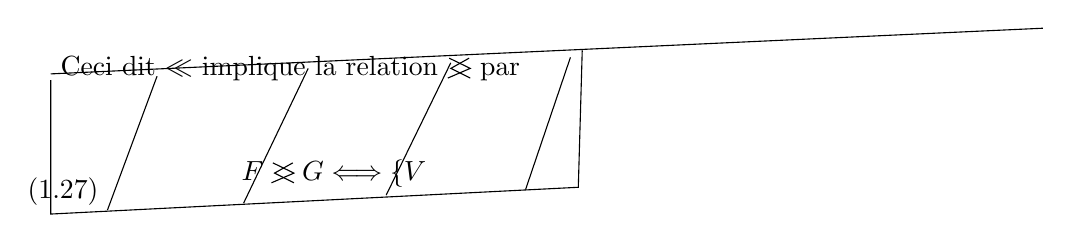
\begin{tikzpicture}[x=1cm,y=1cm]
\node[anchor=west] at (0,1.55) {\deleted{Ceci dit $\ll$ implique la relation $\mathrel{\tikz[baseline=0pt,x=1em,y=1em]{\draw (-.38,.62)--(.38,.25)--(-.43,-.10); \draw (.34,.62)--(-.32,.25)--(.38,-.10);}}$ par}};
\node[anchor=west,inner sep=0pt] at (-.3,-.02) {$\deleted{(1.27)}$};
\node[anchor=west] at (2.3,.22) {$\deleted{F \mathrel{\tikz[baseline=0pt,x=1em,y=1em]{\draw (-.38,.62)--(.38,.25)--(-.43,-.10); \draw (.34,.62)--(-.32,.25)--(.38,-.10);}} G\Longleftrightarrow\{V}$};
\draw (0,1.48)--(12.6,2.06);
\draw (0,1.40)--(0,-.30)--(6.7,.04)--(6.75,1.78);
\draw (.72,-.25)--(1.35,1.45);
\draw (2.45,-.16)--(3.27,1.55);
\draw (4.26,-.06)--(5.08,1.62);
\draw (6.03,.01)--(6.60,1.69);
\end{tikzpicture}}
Je ne vois pas que $\ll$ ($+\ \preccurlyeq$, c'est kif-kif) détermine $\leq$, ni même $\mathrel{\tikz[baseline=0pt,x=1em,y=1em]{\draw (-.38,.62)--(.38,.25)--(-.43,-.10); \draw (.34,.62)--(-.32,.25)--(.38,-.10);}}$. Mais

\textcircled{\unsure{e|$\ominus$}}\quad $\ll$ et $\mathrel{\tikz[baseline=0pt,x=1em,y=1em]{\draw (-.38,.62)--(.38,.25)--(-.43,-.10); \draw (.34,.62)--(-.32,.25)--(.38,-.10);}}$ déterminent $\leq$ par
\margin{$\times$}
\[
G\leq F\quad\unsure{\Longleftarrow|\Longleftrightarrow}\quad (G\ll F\ \text{et}\ G \mathrel{\tikz[baseline=0pt,x=1em,y=1em]{\draw (-.38,.62)--(.38,.25)--(-.43,-.10); \draw (.34,.62)--(-.32,.25)--(.38,-.10);}} F) \tag*{(1.27)}
\]

Donc finalement,

\scanpage{14}\mspage{13}
on trouve comme possibilités \unsure{optima|optimes} de definir la structure d'atelier sur $\unsure{\mathcal{F}|\mathfrak{F}}$ :
\[
\left\{\begin{aligned}
 &\text{Soit par}\quad
 \mathord{\tikz[baseline=(pair.base)]{\node[inner sep=5pt] (pair) {$\leq,\quad\ll$}; \draw ([xshift=1pt]pair.north west)--([xshift=-1pt]pair.north east); \draw ([yshift=-1pt]pair.north east)--([yshift=1pt]pair.south east); \draw ([xshift=-1pt]pair.south east)--(pair.south west)--([yshift=-2pt]pair.north west);}}\\
 &\text{soit par}\quad\leq,\quad\preccurlyeq\\
 &\text{soit par}\quad\ll,\quad
 \mathrel{\tikz[baseline=0pt,x=1em,y=1em]{\draw (-.38,.62)--(.28,.20)--(-.45,-.20); \draw (.35,.52)--(-.30,.18)--(.34,-.18); \draw (-.38,.62)--(-.40,.50)--(.28,.20); \draw (-.30,.18)--(-.42,.08)--(.32,-.14)--(.34,-.23);}}\ .
\end{aligned}\right.
\tag*{(1.28)}
\]
\margin{Non, \unsure{sa|ça} ne suffira pas, \unsure{d'apres|d'après} nouveau point de vue \ldots}

Dans la première mouture, j'ai choisi $\leq$, $\preccurlyeq$, en définissant en termes de ceux-ci
\[
\left\{\begin{aligned}
 &\ll\ \text{est la relation de préordre engendrée par}\\
 &\qquad\leq,\preccurlyeq,\quad \text{ou encore}\\
 &G\ll F\quad\Longleftrightarrow\quad\exists F'\ \text{avec}\quad G\leq F'\preccurlyeq F
\end{aligned}\right.
\tag*{(1.29)}
\]
% slanted
\margin{Je changerai le pt de vue page 20, et ne \unsure{supposerai} plus que $\ll$ soit déterminé ainsi en termes de \unsure{$\leq,\preccurlyeq$,|$\leq,\preccurlyeq$} mais plutôt que $\preccurlyeq$ est déterminé par $\ll,\leq$}

Cela correspond au centre de gravité \deleted{\unsure{conceptuel}} \inserted{\unsure{géometrique|géométrique}} et intuitif, qui est bien sur la notion de subdivision, plutôt que sur celle de raffinement. Mais techniquement c'était un peu laborieux, de déduire les propriétés de transitivité et \inserted{surtout} de \unsure{reflexivité|réflexivité} pour $\ll$, cela amenait à mettre des axiomes en surnombre. Toujours techniquement, il semblerait que ce soit de partir de $\leq,\ll$ qui soit le plus simple. C'est l'approche que je vais suivre tantôt. Quant à la possibilité de passer par $\ll$, $\mathrel{\tikz[baseline=0pt,x=1em,y=1em]{\draw (-.38,.62)--(.38,.25)--(-.43,-.10); \draw (.34,.62)--(-.32,.25)--(.38,-.10);}}$, c'est plutôt une curiosité qu'autre chose,

\scanpage{15}\mspage{14}
En résumé, en termes de $\unsure{\mathcal{F}|\mathfrak{F}}$, c'est de la donnée de deux \uline{relations} \uline{d'ordre}
% The enclosure has separate top, left and bottom strokes; no right vertical is visible.
\figure{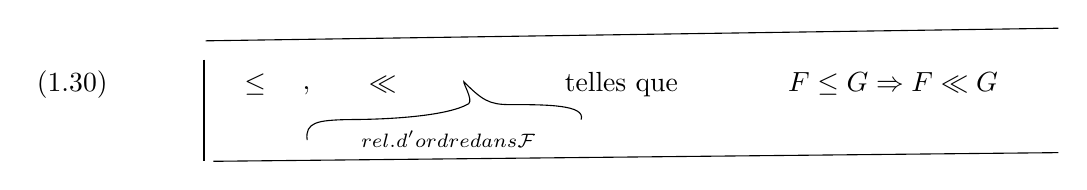
\begin{tikzpicture}[x=1cm,y=1cm]
  \node[anchor=east] at (-1.1,0.68) {$(1.30)$};
  \node at (0.65,0.68) {$\leq$};
  \node at (1.30,0.59) {$,$};
  \node at (2.27,0.68) {$\ll$};
  \node at (5.30,0.68) {telles que};
  \node at (8.75,0.68) {$F\leq G\Rightarrow F\ll G$};
  \node at (3.10,-0.02) {$\scriptstyle\text{rel. d'ordre dans }\mathcal{F}$};
  \draw (0.02,1.23) -- (10.85,1.39);
  \draw (0,0.99) -- (0,-0.30);
  \draw (0.12,-0.30) -- (10.85,-0.19);
  \draw (1.31,-0.03) .. controls (1.28,0.20) and (1.45,0.22) .. (1.82,0.23)
    .. controls (2.40,0.23) and (3.10,0.28) .. (3.36,0.43)
    .. controls (3.42,0.48) and (3.29,0.69) .. (3.30,0.71)
    .. controls (3.53,0.48) and (3.62,0.42) .. (3.88,0.42)
    .. controls (4.34,0.42) and (4.85,0.42) .. (4.79,0.23);
\end{tikzpicture}}
que je vais partir.

En termes de celles-ci, on definit \deleted{$\unsure{\mathcal{M}|M}$}
\[
\mathcal{M}\subset\mathcal{F}
\]
par (1.20), \unsure{avec} les relations $\underset{\mathcal{M}}{\leq},\ \underset{\mathcal{M}}{\ll}$ induites par $\underset{\mathcal{F}}{\leq},\ \underset{\unsure{\mathcal{F}|\overline{f}}}{\ll}$, puis
\[
\mathcal{L}\subset\mathcal{M}
\]
par (1.25). L'application
\[
\mathcal{F}\hookrightarrow\unsure{\mathcal{P}|\mathscr{P}|\mathfrak{P}}(\mathcal{M})\qquad
\mathord{\rlap{$\deleted{X}$}F}\longmapsto\widetilde F=\mathrm{Dep}(F)
\tag*{($*$)}
\]
% The input X is overwritten by F at the same horizontal position.
est \inserted{alors} definie par
\[
\widetilde F=\{X\in\mathcal{M}\mid X\leq F\}
\tag*{(1.31)}
\]
et
\[
\mathcal{F}\hookrightarrow\mathrm{Fig}(\mathcal{M})\qquad
\unsure{F|\deleted{F}|\mathord{\rlap{$\deleted{X}$}F}}\longmapsto\mathrm{Fig}_{\mathcal{M}}(F)
\tag*{($**$)}
\]
% At the second map an extra diagonal crosses F; live F, canceled F, and X overwritten by F remain possible.
par (1.4) :
\[
\mathrm{Fig}_{\mathcal{M}}(F)=\{\widetilde X\mid X\in\widetilde F\}\subset\mathcal{P}(\mathcal{M})
\tag*{\deleted{(1.32)}}
\]
avec
\[
\widetilde X=\{Y\in\mathcal{M}\mid Y\leq X\}\quad.
\]

Ainsi, $\mathcal{F}$ est interprété comme un ens. de parties dans $\mathcal{M}$ via ($*$), et $\leq$ \unsure{s'interprète|s'interprête} simplement par l'inclusion
\[
F\leq G\Longleftrightarrow\widetilde F\subset\widetilde G
\tag*{(1.32)}
\]
